% Capítulo 9: as chamadas de fatorial(4) descendo e as respostas voltando.
\documentclass[border=4pt]{standalone}
\usepackage[utf8]{inputenc}
\usepackage[T1]{fontenc}
% Estilo comum dos fluxogramas e diagramas de blocos.
\usepackage{tikz}
\usetikzlibrary{arrows.meta, positioning, calc, shapes.geometric, shapes.misc}
\definecolor{navy}{RGB}{23,45,80}
\definecolor{laranja}{RGB}{250,110,29}
\definecolor{cinzalogo}{RGB}{107,114,126}
\definecolor{azul}{RGB}{205,222,247}
\tikzset{
  base/.style={draw=navy, line width=0.9pt, font=\sffamily\small, align=center, inner sep=4pt},
  terminal/.style={base, rounded rectangle, fill=laranja!45, draw=laranja, minimum width=20mm, minimum height=7mm},
  processo/.style={base, rectangle, fill=laranja!12, minimum width=28mm, minimum height=8mm},
  decisao/.style={base, diamond, aspect=2.2, fill=azul, inner sep=1pt, minimum width=30mm},
  es/.style={base, trapezium, trapezium left angle=72, trapezium right angle=108,
             fill=white, minimum width=26mm, minimum height=8mm, trapezium stretches body},
  fluxo/.style={-{Stealth[length=2.2mm]}, navy, line width=0.9pt},
  rotulo/.style={font=\sffamily\small\bfseries, text=navy},
  legenda/.style={font=\sffamily\scriptsize, text=cinzalogo},
  resposta/.style={font=\sffamily\scriptsize\bfseries, text=navy},
}

\tikzset{
  chamada/.style={base, rectangle, rounded corners=2pt, fill=azul, font=\ttfamily\small, minimum width=46mm, minimum height=7mm},
  basecaso/.style={chamada, fill=laranja!45, draw=laranja},
  volta/.style={-{Stealth[length=2.2mm]}, laranja, line width=0.9pt},
  valor/.style={font=\sffamily\small\bfseries, text=laranja},
}
\begin{document}
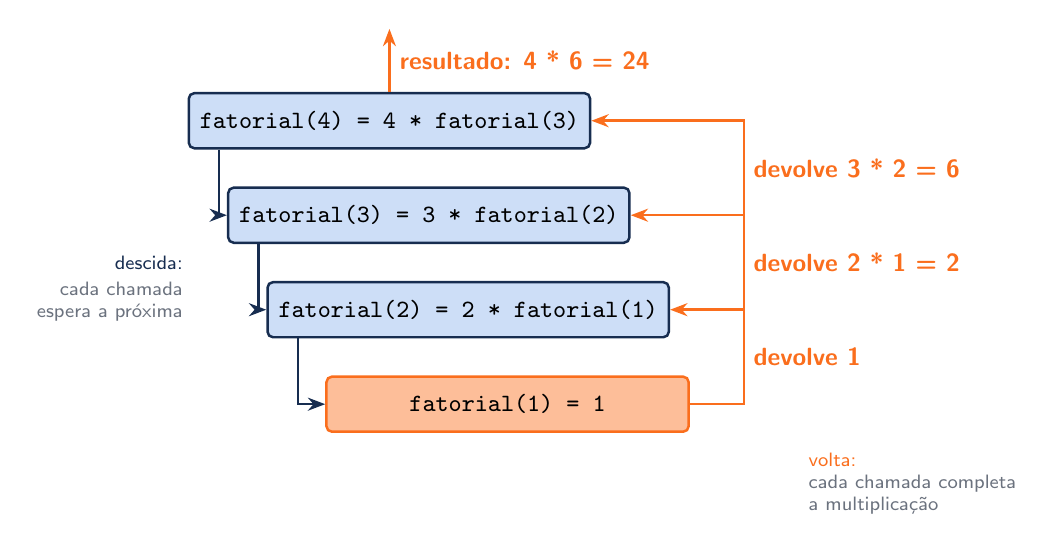
\begin{tikzpicture}
  \node[chamada] (c4) at (0, 0) {fatorial(4) = 4 * fatorial(3)};
  \node[chamada] (c3) at (0.5, -1.2) {fatorial(3) = 3 * fatorial(2)};
  \node[chamada] (c2) at (1.0, -2.4) {fatorial(2) = 2 * fatorial(1)};
  \node[basecaso] (c1) at (1.5, -3.6) {fatorial(1) = 1};
  \draw[fluxo] ($(c4.south west)+(0.4, 0)$) |- (c3.west);
  \draw[fluxo] ($(c3.south west)+(0.4, 0)$) |- (c2.west);
  \draw[fluxo] ($(c2.south west)+(0.4, 0)$) |- (c1.west);
  \draw[volta] (c1.east) -- (4.5, -3.6) |- (c2.east);
  \draw[volta] (4.5, -2.4) |- (c3.east);
  \draw[volta] (4.5, -1.2) |- (c4.east);
  \node[valor, right] at (4.5, -3.0) {devolve 1};
  \node[valor, right] at (4.5, -1.8) {devolve 2 * 1 = 2};
  \node[valor, right] at (4.5, -0.6) {devolve 3 * 2 = 6};
  \draw[volta] (c4.north) -- node[valor, right] {resultado: 4 * 6 = 24} ++(0, 0.8);
  \node[legenda, text=navy, anchor=east] at (-2.5, -1.8) {descida:};
  \node[legenda, anchor=east, align=right] at (-2.5, -2.3) {cada chamada\\espera a próxima};
  \node[legenda, text=laranja, anchor=west] at (5.2, -4.3) {volta:};
  \node[legenda, anchor=west, align=left] at (5.2, -4.75) {cada chamada completa\\a multiplicação};
\end{tikzpicture}
\end{document}
